\documentclass{sig-alternate-10pt}

\usepackage{url, enumitem}

\begin{document}

\title{RaptorQ-based File Transfer Protocol}
\author{
  Yilong Li\\
  \texttt{yilongl@cs.stanford.edu}
  \and 
  Raejoon Jung\\
  \texttt{raejoon@stanford.edu}
  \and
  Yu Yan\\
  \texttt{yuyan0@stanford.edu}
}

\maketitle
\section{Introduction}

\section{Implementation}

\subsection{Reliable file transfer}

In Tornado transfer, the reliability guarantee is achieved at the application level by the use of RaptorQ code. This eliminates the need for retransmission at the file transfer application level, which greatly simplifies the design and implementation of a reliable file transfer protocol. In Tornado transfer, the sender has no need to keep track of exactly what symbols are received by the receiver. Therefore, the ACK message is essentially just a bitmask of 256 bits (256 is the maximum number of blocks specified in RFC6330) that records which blocks have been successfully decoded by the receiver. Tornado transfer protocol has a handshake procedure similar to TCP to establish the connection. Once the handshake succeeds, the sender starts sending source symbols of each block in order. Furthermore, in order to compensate for the potential lost symbols, the sender sends one repair symbol for each previously un-ACK'ed block after every X source symbols. After all source symbols have been sent, the sender simply sends repair symbols for each un-ACK'ed block in a round-robin fashion. Ideally, the repair symbol transmission interval X should be set to a value such that after all source symbols of block n has been sent, the receiver has received enough symbols for block n-1 for decoding. This way, the receiver only needs to keep roughly one block in memory for decoding at a time. The receiver sends back a heartbeat ACK message constantly to compensate for potentially lost ACK messages. Besides, it immediately sends back an ACK message once it decodes a new block to reduce the probablity of sender sending more symbols for the decoded blocks. Once the receiver decodes the entire file, it simply exits. The sender will also terminate once it figures out that the receiver exits. This can be done either by relying on the shutdown mechnaism of DCCP socket or through an ICMP destination unreachable message generated by the receiver.

Parameter setting
There are two most important paramenters that we can pass on to the RaptorQ library: symbol size and number of symbols per block.

1. Symbol size
In our current implementation, we choose the symbol size to be 1400 bytes to avoid IP fragmentation. We could potentially choose a larger number to, say, reduce the number of symbols for performance reason described in the section below. However, the downside of a larger symbol size is that each symbol may be fragmented at the IP layer and the loss of each fragment results in the loss of the entire symbol. In other words, the nice property of digital fountain that every packet received contributes to the decoding of the entire file is no longer preserved. Currently, we have not quantified the effect of a larger symbol size.

2. Number of symbols per block
The number of symbols per block is critical to the performance of encoding and decoding. Generally speaking, we would like to keep it as small as possible. RFC 6330 does not allow us to explicitly set this value. Instead, we provide a parameter WS, the maximum size of a block that can be efficiently decoded in the working memory of the receiver, and RFC 6330 describes the procedure for deriving the number of symbols per block based on it. This parameter derivation algorithm involves lookups into the hardcoded RaptorQ matrices and is not very straightforward. Therefore, our current implementation enumerates paramenter WS starting from a small number and increase it by one each time to search for the smallest legal value of the number of symbols per block. In pratice, this search procedure is fast enough to be hardly notieable.

Performance bottlenecks
Our current implementation of Tornado transfer has two performance bottlenecks which limits its practicality. We briefly describe the problems here and leave the solutions as future work.

1. Precomputation
The most computational expensive in RaptorQ encoding/decoding process is the process of precomputing intermediate symbols for each block. The time complexity of the precomputation is cubic in the number of symbols per block. We currently use a background thread for precomputing intermediate symbols while transmitting symbols. However, this has become a bottleneck for larger file size. For instance, for a file of size 100MB, the smallest number of symbols per block that is legal with respect to RFC 6330 is 296.

2. Decoding
Once intermediate symbols have been precomputed, even though both encoding and decoding are linear in the number of symbols, decoding tends to fall behind encoding for two reasons. First, encoding is a stream operation that takes constant time to generate the next symbol, while decoding is a batch operation that only happens after enough symbols of a block have been received. Second, decoding is inherently slower than encoding in the current implementation of libRaptorQ. To resolve this bottleneck, 
\subsection{Congestion control}

\section{Evaluation}
We test the tornado transfer implementation using emulated links generated by
Mahimahi \cite{mahimahi}. We measure the time spent for sending a file through
mahimahi with various link parameters. File transfer time via SCP is also
measured and compared. We observe the transfer time while changing three
parameters: (1) link loss, (2) link delay, and (3) file size. We fix the link
bandwidth to 12 Mbps. For each set of parameters, we ran 10 tests and report the
mean and the standard deviation in the following plots.

\subsection{Link loss test}

\begin{figure}[t]
  \centering
  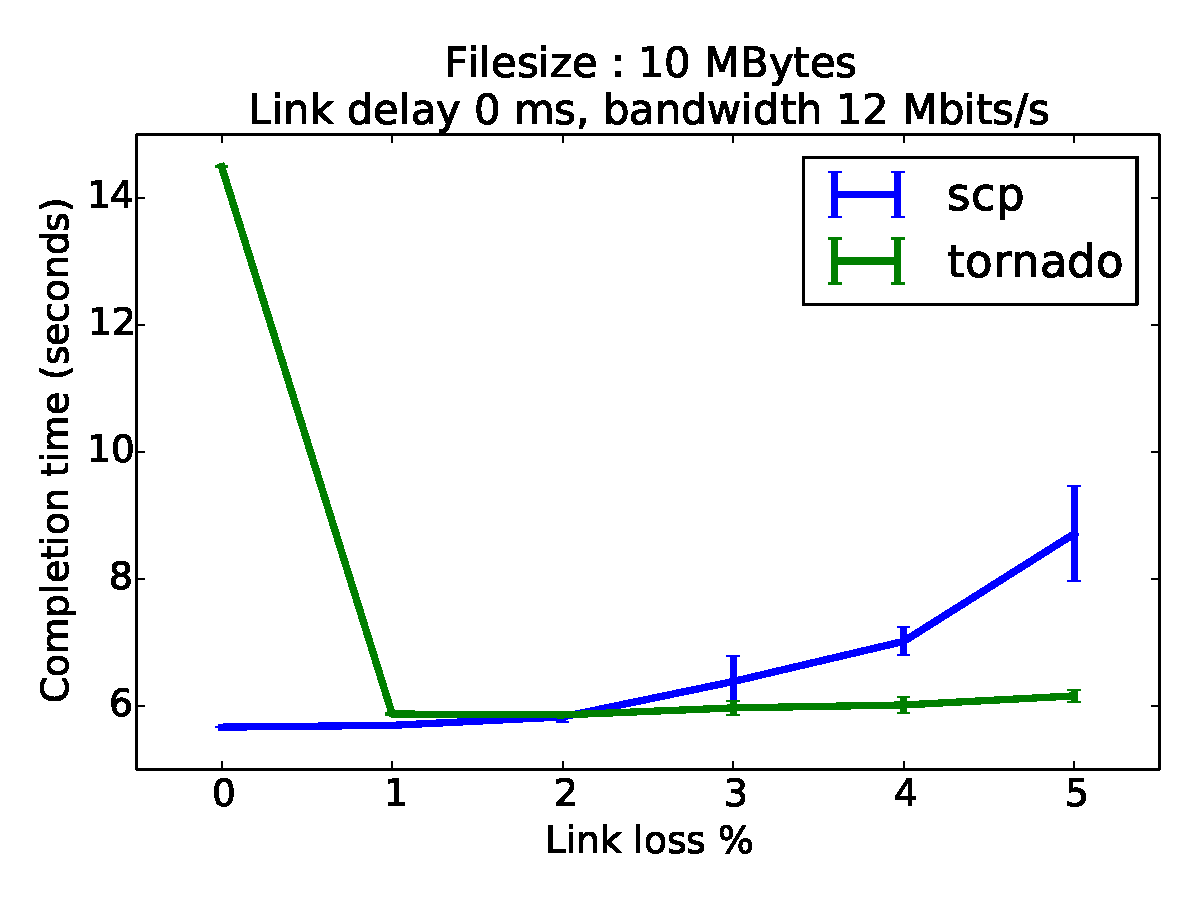
\includegraphics[width=0.5\textwidth]{loss-plot}
  \caption{Transfer time in lossy link}
  \label{f:loss-plot}
\end{figure}

Figure \ref{f:loss-plot} depicts the file transfer time using Tornado and SCP in
links with various packet loss probabilities. When the loss probability is
$\geq$ 1\%, transfer time of Tornado and SCP monotonically increase as the loss
probability increases. However the growth of Tornado's transfer time is much
less than SCP's transfter time. This results in a faster transfer time with
Tornado in loss proabilities of $\geq$ 2\% and the gap between the transfer time
of the two protocols gets wider as the loss proability increases.A

One interesting fact that we noticed is the transfer time using Tornado when
the loss probability is 0, i.e., the link is lossless. The average transfer time of
Torndao exceeds 14 seconds which is greater than $2\times$ compared to the case
when the link has 1\% loss probability. This is counter-intuitive since we
expect that packet loss can only deteriorate the operation of the file transfer
protocol. Currently, we do not have a clear explanation of this observation and
leave to future work to enhance the implementation to gracefully degrade
performance as the link probability increases.


\subsection{Link delay test}

\begin{figure}[t]
  \centering
  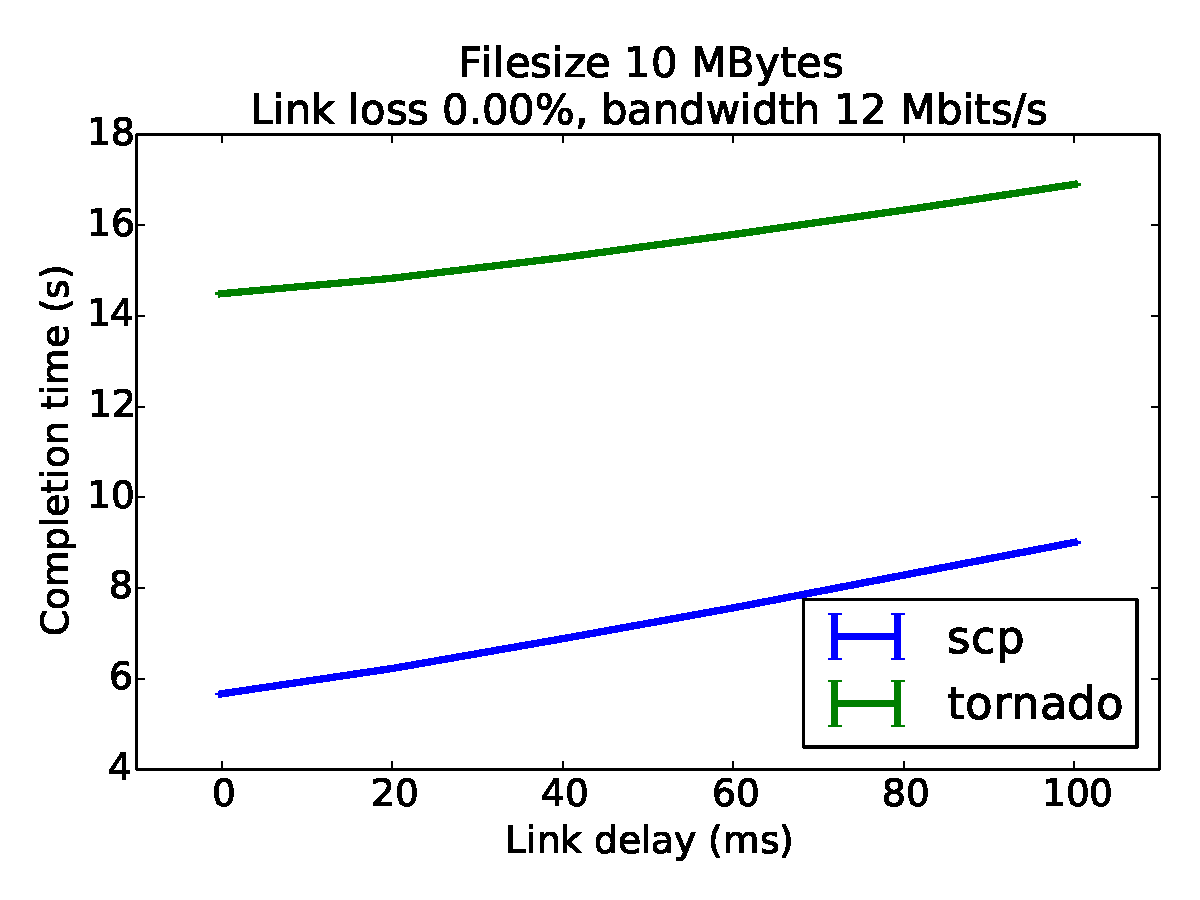
\includegraphics[width=0.5\textwidth]{delay-plot}
  \caption{Transfer time in link with delay. One way delays are stated.}
  \label{f:delay-plot}
\end{figure}

Figure \ref{f:delay-plot} shows the file transfer time in links with various
delay values. Throughout delay values from 0 to 100 ms, SCP maintains $\sim
2\times$ performance of Tornado. However, the difference of the transfer time is
almost constant in this delay range. In fact, the difference slightly decreases
as the delay increases. 

We first suspected the stage of computing intermediate symbols in Tornado to
cause this diffrence since this portion of the protocol requires extensive
computation and is done before the datagram transfer loop.  However, we have
confirmed that the progress of sending datagram was widely spread across the
application runtime rather than having a burst of datagram transfers after a
long pause as we expect if the intermediate symbol computation was the
bottleneck. From this observation, we expect this difference comes from the
inefficiency of our implmentation of the datagram transfer loop rather than
caused by the inefficiency of the design of the protocol.

\subsection{File size test}

\begin{figure}[t]
  \centering
  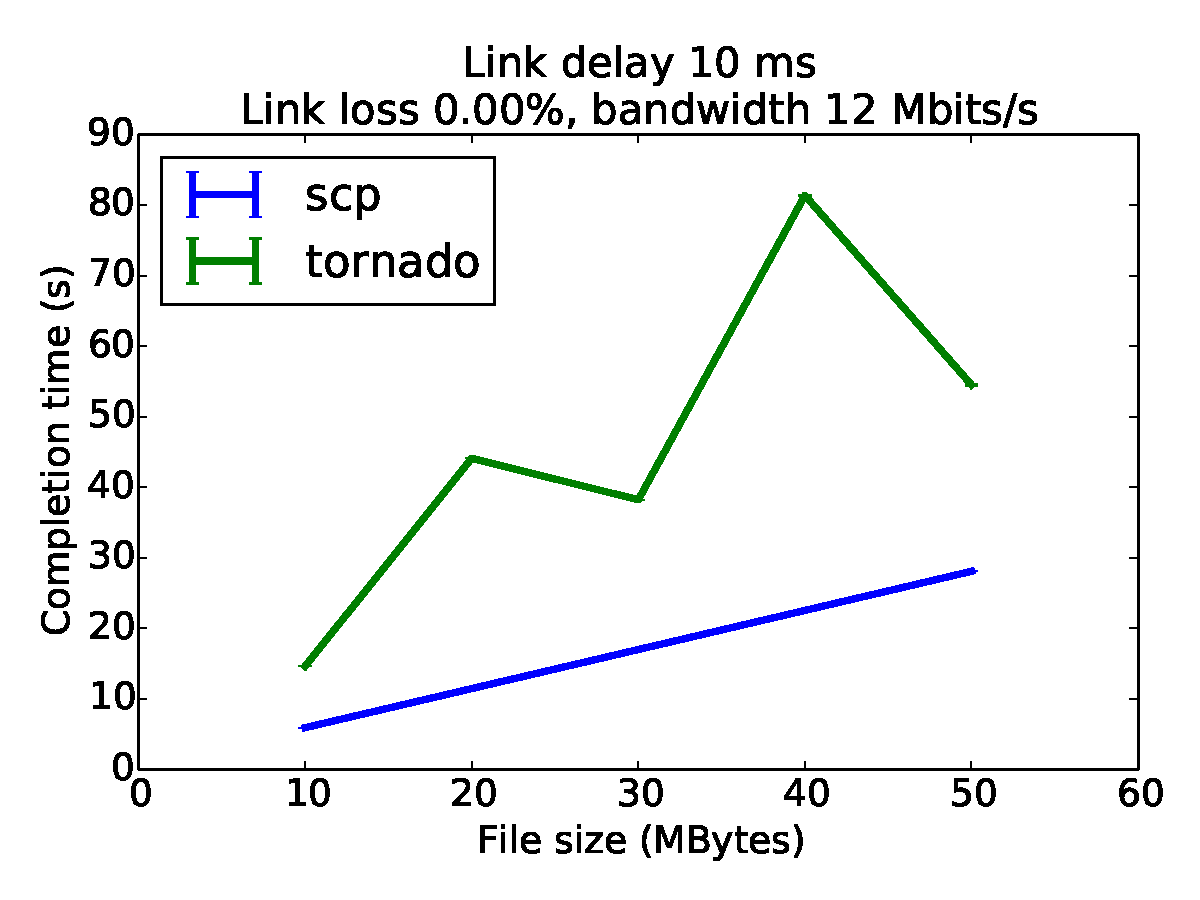
\includegraphics[width=0.5\textwidth]{filesize-plot}
  \caption{Transfer time with various file sizes}
  \label{f:filesize-plot}
\end{figure}

Figure \ref{f:filesize-plot} depcits the file transfer time using Tornado and
SCP with various file sizes when the link is lossless and has a one-way delay of
10ms. We tested with file sizes of 10, 20, 30, 40, and 50 MBs. In this range,
SCP transfers files faster than Tornado. Eventhough Tornado's transfer time does
not monotonically increase as the file size increases, the difference between
the transfer time of SCP and Tornado tends to increase.

The fact that Tornado's transfer time not increasing monotonically is also
noteworthy. We suspect that this is caused by the \texttt{libRaptorQ}'s internal
decision to set the number of blocks given a file size. Since we have no control
on the number of symbols per block since the size of a block can change
depending on \texttt{libRaptorQ}'s decision while we fix the symbol size. For
improvement, we can split the file into subfiles of fixed size and feed them
into multiple instances of encoders. Then we can expect regular performance
throughout the encoders. We leave the validation of the hypothesis and the
improvement for future work.

\section{Contribution}

\section{Reflection}

\section{Conclusion}

\cite{openrq}

\bibliography{finalreport}
\bibliographystyle{acm}

\end{document}
